\documentclass[11pt,letterpaper]{article}
\usepackage[lmargin=1in,rmargin=1in,tmargin=1in,bmargin=1in]{geometry}
\usepackage{../style/homework}
\usepackage{../style/commands}
\setbool{quotetype}{true} % True: Side; False: Under
\setbool{hideans}{true} % Student: True; Instructor: False

% -------------------
% Content
% -------------------
\begin{document}

\homework{15: Due 11/16}{He is a self-made man and worships his creator.}{Henry Clapp}

% Problem 1
\problem{10} As accurately as possible, plot the function $f(x)= \frac{1}{4} \left( 2^{x - 2} \right)$.
	\[
	\fbox{
	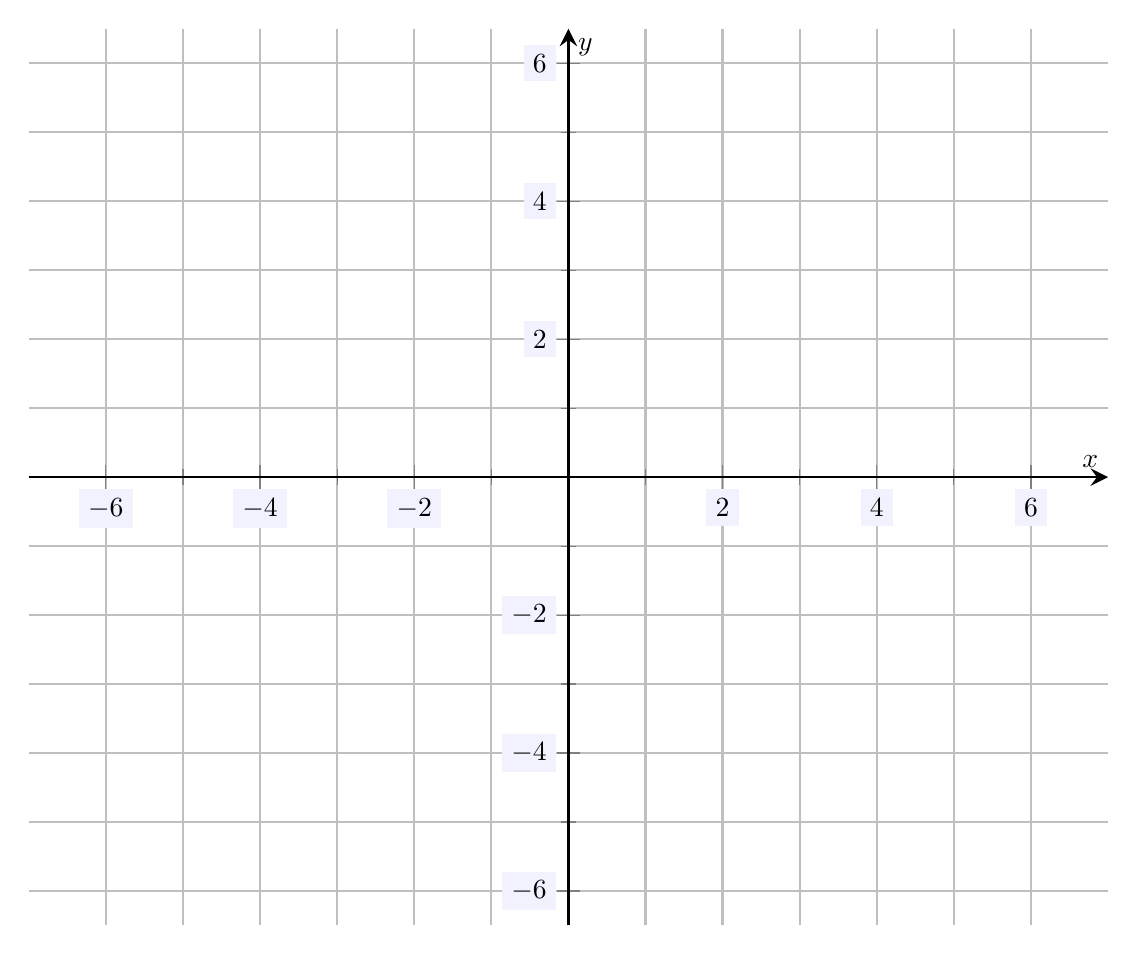
\begin{tikzpicture}[scale=2,every node/.style={scale=0.5}]
	\begin{axis}[
	grid=both,
	axis lines=middle,
	ticklabel style={fill=blue!5!white},
	xmin= -7, xmax=7,
	ymin= -6.5, ymax=6.5,
	xtick={-6,-4,-2,0,2,4,6},
	ytick={-6,-4,-2,0,2,4,6},
	minor tick = {-5,-3,...,5},
	xlabel=\(x\),ylabel=\(y\),
	]
	\end{axis}
	\end{tikzpicture}
	}
	\] \pspace





\newpage





% Problem 2
\problem{10} Sketch a graph of the function $y= 4 (2^{1 - x})$. 
	\[
	\fbox{
	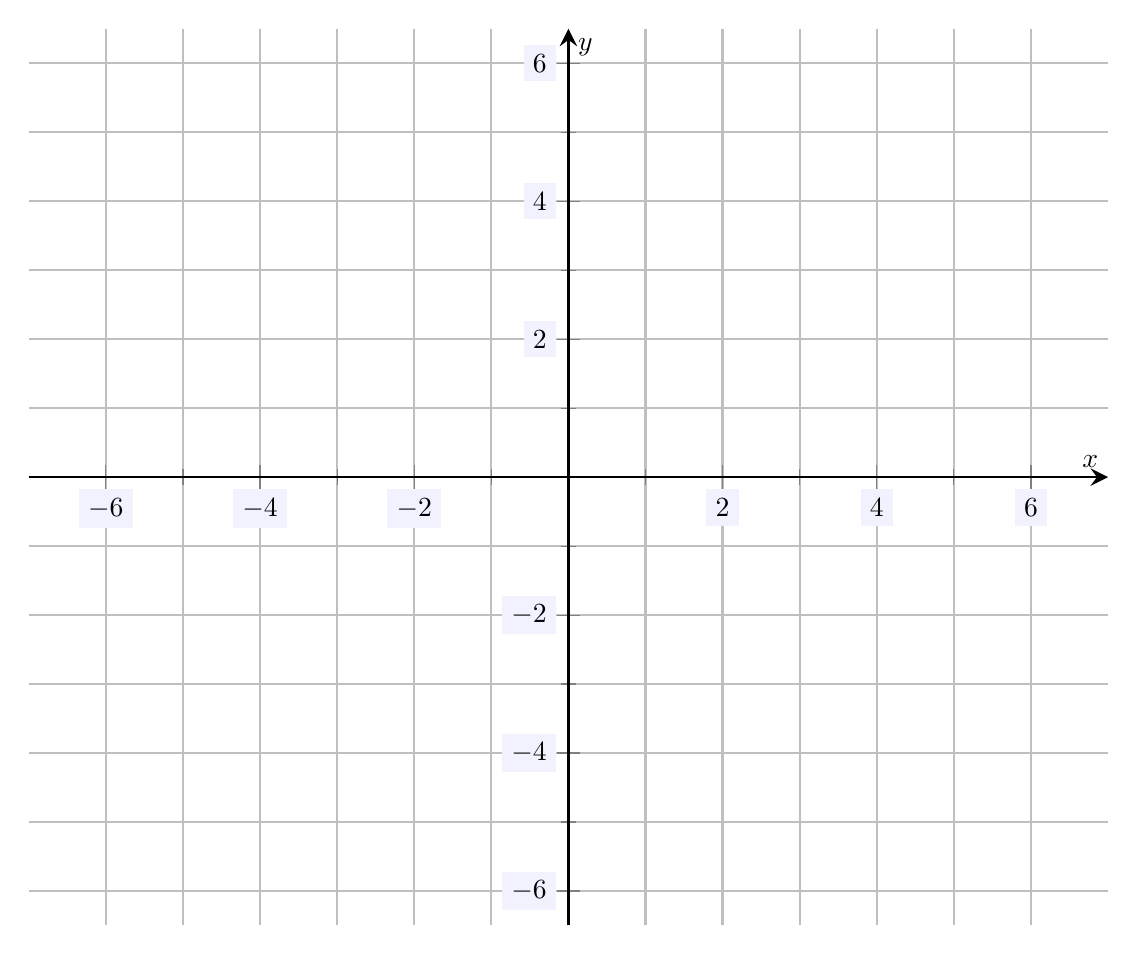
\begin{tikzpicture}[scale=2,every node/.style={scale=0.5}]
	\begin{axis}[
	grid=both,
	axis lines=middle,
	ticklabel style={fill=blue!5!white},
	xmin= -7, xmax=7,
	ymin= -6.5, ymax=6.5,
	xtick={-6,-4,-2,0,2,4,6},
	ytick={-6,-4,-2,0,2,4,6},
	minor tick = {-5,-3,...,5},
	xlabel=\(x\),ylabel=\(y\),
	]
	\end{axis}
	\end{tikzpicture}
	}
	\] \pspace





\newpage





% Problem 3
\problem{10} Consider the function $y= -9 (2^{-2x})$.
\begin{enumerate}[(a)]
\item Is the function increasing or decreasing? Explain.
\item Find the $y$-intercept of this function.
\item What are the $x$-intercepts and zeros for this function?
\item Find $y(-1)$. 
\end{enumerate} \pspace





\newpage





% Problem 4
\problem{10} Consider the function $y= 3^{1-x} - 9$.
\begin{enumerate}[(a)]
\item Is the function increasing or decreasing? Explain.
\item Find the $y$-intercept of this function.
\item What are the $x$-intercepts and zeros for this function?
\item Find $y(2)$. 
\end{enumerate} \pspace


%\printpoints
\end{document}